\documentclass[11pt]{article}

%\usepackage{pslatex}
\usepackage{apacite}
\usepackage{amsmath,amssymb}
\usepackage{graphicx}
\usepackage{color}
\usepackage{url}
\usepackage{fullpage}
\usepackage{setspace}
\usepackage{booktabs}
%\newcommand{\url}[1]{$#1$}


\definecolor{Red}{RGB}{255,0,0}
\newcommand{\red}[1]{\textcolor{Red}{#1}}

 \newcommand{\denote}[1]{\mbox{ $[\![ #1 ]\!]$}}


\newcommand{\subsubsubsection}[1]{{\em #1}}
\newcommand{\eref}[1]{(\ref{#1})}
\newcommand{\tableref}[1]{Table \ref{#1}}
\newcommand{\figref}[1]{Figure \ref{#1}}
\newcommand{\appref}[1]{Appendix \ref{#1}}
\newcommand{\sectionref}[1]{Section \ref{#1}}

\doublespacing

\title{Wonky worlds: Listeners revise world knowledge when utterances are odd}
%\title{Wonky worlds: Listeners reconsider world knowledge when utterances are odd}
%Non-sinking marbles are wonky: defeasible world knowledge in language interpretation}

 
\author{{\large \bf Judith Degen, Michael Henry Tessler, Noah D.~Goodman} \\
  \{jdegen,mhtessler,ngoodman\}@stanford.edu\\
  Department of Psychology, 450 Serra Mall \\
  Stanford, CA 94305 USA}

% ggplot colors: "#F8766D", "#A3A500", "#00BF7D", "#E76BF3", "#00B0F6"

% variations on blue: "#007fb1", "#4ecdff"


%% TODO
% somewhere in the intro, discuss what other theories of scalar implicature/utterance interpretation have to say about world knowledge 
% add Exp. 4 (run it first...)
% rework discussion
% add appendix with all items

% in intro (or discussion?) talk about what other people have said about how world knowledge is integrated in utterance interpretation, and data that shows that it does. e.g., from guerts (2010, p. 78) : "In general, a sentence like �The peanut was in love�, would yield a massive N400 for the last word. But what will happen when this sentence is embedded in a discourse like the following: 'A woman saw a dancing peanut who had a big smile on his face. The peanut was singing about a girl he had just met. And judging from the song, the peanut was totally crazy about her. The woman thought it was really cute to see the peanut singing and dancing like that. The peanut was {salted/in love}, and by the sound of it, this was definitely mutual. He was seeing a little almond.' (Nieuwland and van Berkum 2006: 1106) As reported by Nieuwland and van Berkum, in this context it is �salted�, not �in love�, that elicits an N400. Apparently, the expectations tracked by the N400 take into account contextual information, as well as general world knowledge. One of the most salient components of the context is the speaker, and van Berkum et al. (2008) showed that the N400 takes into account information about the speaker, too. In van Berkum et al.�s study, people listened to sen- tences whose meanings might be at odds with reasonable assumptions about the speaker�s sex, age, or social status, as inferred from the speaker�s voice. For example, when �I have a large tattoo on my back� was spoken in an upper- class accent, there was an obvious discrepancy between social elevation and dorsal decoration, which became apparent at the critical word �tattoo�. This type of mismatch, too, turned out to yield an N400."

\begin{document}

\maketitle


\begin{abstract}
\red{World knowledge enters into pragmatic utterance interpretation in complex ways, and may be defeasible in light of speakers' utterances.  Yet there is to date a surprising lack of systematic investigation into the role of world knowledge in pragmatic inference. In this paper, we show that a state-of-the-art model of pragmatic interpretation greatly overestimates the influence of world knowledge on the interpretation of utterances like \emph{Some of the marbles sank}. We extend the model to capture the idea that  the listener is uncertain about the background knowledge the speaker is bringing to the conversation. This extension greatly improves model predictions of listeners' interpretation and also makes good qualitative predictions about listeners' judgments of how `normal' the world is in light of a speaker's statement. Theoretical and methodological implications are discussed.}


\textbf{Keywords:} 
scalar implicature; world knowledge; prior beliefs; experimental pragmatics; computational pragmatics
\end{abstract}

\section{Introduction}
\label{sec:intro}

How often do you think marbles sink in water? Probably extremely often, if not always. Now imagine someone says \emph{Max threw fifteen marbles in the water. Some of the marbles sank.} Have you begun to reconsider your assumptions? Perhaps you now suspect that these marbles are in fact made of hollow plastic or the water is covered with thick algae? That is, maybe you have begun to suspect that these are not just normal marbles in normal water. Alternatively, maybe you know the speaker who produced the utterance and know them to be unreliable in their descriptions of the world. Here we explore how prior world knowledge enters into pragmatic utterance interpretation, and when this world knowledge is defeasible: some utterances are odd and may lead listeners to conclude that the world under discussion is abnormal in the sense that events in that world have appropriately different prior probabilities. We refer to such abnormal worlds  as \emph{wonky} worlds. However, sometimes the oddness of those same utterances may be explained away by the knowledge of \emph{speaker unreliability}, in which case listeners' prior beliefs about the world that they bring to bear on the utterance situation should remain unchanged.

The Rational Speech Act framework  \cite<RSA, >{frank2012,goodmanstuhlmueller2013}, and related models \cite{franke2011,russell2012}, treat communication as a signaling game \cite{lewis1969} between a speaker and a listener.
The listener reasons by Bayesian inference about what the world is like given that a speaker who produced the utterance is trying to be informative (with respect to a na\"ive listener who interprets utterances literally). 
Variants of these models have successfully captured listeners' quantitative  behavior on a number of pragmatic inference tasks, including ad hoc Quantity implicature \cite{degenfrankejaeger2013}, markedness implicature \cite{bergengoodman2012}, scalar implicature \cite{goodmanstuhlmueller2013}, syllogistic reasoning \cite{tessler2014}, and non-literal language \cite{kao2014}. 
A defining feature of Bayesian reasoning is that prior beliefs affect inferences that will be drawn. Bayesian models of language interpretation, accordingly, predict that prior beliefs about the world should affect the listener's interpretation of an utterance. 
%These models make clear predictions about how prior beliefs about states of the world should be integrated with listeners' expectations about utterances a speaker is likely to produce to communicate a particular state of the world. 
While this impact of prior knowledge has been noted, and included in models, it hasn't been systematically studied.

Generalizing our opening example, consider \emph{Some of the X sank}, where \emph{X} is a plural noun such as \emph{marbles}, \emph{feathers}, or \emph{balloons}, and \emph{the X} refers to a contextually established group of objects from category X. When the prior probability, $\theta_{X}$, of an X\footnote{We will use `X' interchangeably to refer to both the category and the members of the category.} sinking is not extreme (e.g., a feather sinking), RSA leads to the standard scalar implicature: the posterior probability that all of the X sank, after hearing the utterance, is much lower than its prior probability (i.e., \emph{Some of the feathers sank} yields that not all of them did). This is because a rational speaker would have been expected to produce the more informative (and contextually relevant) \emph{All of the X sank}, had it been true.
As we will show in \sectionref{sec:rsa}, RSA makes two strong predictions about the effect of the prior on the interpretation of \emph{Some of the X sank}: 

\begin{enumerate}
	\item As $\theta_{X}$ approaches $1$, the interpretation probability that all X sank approaches $1$, that is, the scalar implicature disappears. 
This prediction follows because the extreme prior overwhelms the effect of the  utterance's semantics.
	\item For moderate to high prior probability (roughly $0.5{<}\theta_{X}{<}1$) and a large total number of objects (more than about 10), the posterior expectation of the number of X that sank should be approximately the same as the prior expectation---that is, the utterance shouldn't affect the expected number of X that sank. 
\end{enumerate}
	
%
These predictions follow from the weak semantics of \emph{some} and the isolated effect of the alternative \emph{all}: \emph{Some of the X sank} only restricts the interpretation (i.e., the number of X that sank) to be greater than zero; competition with \emph{All of the X sank} results in the scalar implicature that can at most rule out the state in which all of the X sank. But that leaves at least fourteen other possibilities: that one X sank, that two X sank, etc. Thus, a sufficiently strong prior will dominate the inference about exactly how many X sank.

% JUDITH'S SUPER SENTENCE THAT EVERYONE ELSE HATES:
%This prediction follows from the weak semantics of \emph{some} and the isolated effect of the alternative \emph{all}: because \emph{Some of the X sank} only restricts the interpretation (i.e., the number of marbles that sank) to be greater than zero, and because the scalar implicature resulting from the alternative \emph{All of the X sank} can at most rule out the state in which all of the X sank, the prior will dominate the inference about exactly how many X sank.


However, intuition is at odds with these predictions: as \citeA{geurts2010} has observed, for events with very high prior probability of occurrence (e.g., marbles sinking), observing an utterance such as \emph{Some of the marbles sank} seems to yield strong implicatures; that is, contrary to RSA predictions, the subjective probability that all of the marbles sank is intuitively close to 0. 
%The reason for this is presumably that listeners realize that the speaker went to the trouble of producing an utterance that is weaker than what the prior would lead one to believe.
%

The rest of the paper is structured as follows. In Exp.~1 we collect prior probabilities for a variety of events (e.g., sinking) and categories that participate in those events (e.g., marbles). In Exps.~2a and 2b we collect corresponding posterior interpretations after observing descriptions of those events containing quantifiers (\emph{some}, \emph{all}, \emph{none}). These experimental results confirm the intuition of relatively strong implicatures---hence prediction (1) of RSA is incorrect---and show that the prior has a muted effect on posterior expectation---hence prediction (2) of RSA is incorrect.

Given the previous success of RSA models, this constitutes a striking puzzle. 
To address this puzzle we pursue the intuition raised at the very beginning of this paper: that sometimes, the speaker's utterance will lead the listener to infer that the world under discussion is wonky and she should therefore use less extreme prior beliefs in the computation of speaker meaning. In \sectionref{sec:wrsa} we introduce a variant of RSA, \emph{wonky RSA (wRSA)}, in which the listener can revise her beliefs about the domain under discussion. We show that this extension resolves the puzzle of the prior's muted effects.

The extended wRSA model makes predictions not just about the actual state of the world that the listener infers the speaker as trying to communicate, but also about listeners' judgments of world wonkiness. This allows for a further test of wRSA: in Exp.~3 we collect participants' judgments about whether the world is wonky in the scenarios of Exps.~2a and 2b.

Finally, in \sectionref{sec:speakerreliability} we test the prediction that listeners should hold on to their prior beliefs when interpreting odd utterances if they expect  speakers to be  unreliabile. That is, if utterance oddness can be explained away by speaker unreliability, prior beliefs about how many X Y should have a greater effect on the interpretation of \emph{Some of the X Yed} than when speakers are expected to be reliable. We test the effect of speaker reliability on interpretation of a subset of the items used in Exps.~2a-3 in Exp.~4. In \sectionref{sec:gd} we discuss the results with respect to a) ideal adaptor models in other areas of psycholinguistics and b) presupposition accommodation / common ground update.


\section{Experiment 1a and 1b: prior elicitation} 
\label{sec:priors}

Obtaining good estimates of prior beliefs is crucial for testing any Bayesian model. Indeed, Bayesian approaches have recently been criticized for being lax in their treatment of priors \cite{jones2011, marcus2013}. To avoid this criticism, we would thus like to obtain good empirical estimates of prior beliefs. A problem in this endeavor is that there are no clearly established dependent measures for eliciting prior beliefs about different types of events. One way to solve this problem is to elicit priors using different dependent measures and using the data obtained in this way to infer the underlying `true' prior. This is what we do here. Exp.~1a and 1b\footnote{These experiments can be viewed at \url{http://cocolab.stanford.edu/cogsci2015/wonky/prior/sinking-marbles-prior.html} and \url{http://cocolab.stanford.edu/cogsci2015/wonky/prior_sliders/sinking-marbles.html}.} measured listeners' prior beliefs about how many objects exhibit a certain effect (e.g., how many marbles sink) using two different dependent measures. The `true' prior that is used in all subsequent analyses throughout the paper was then inferred by \red{XXX MH summarize procedure in one sentence}.

\subsection{Method}

\subsubsection{Participants}
For each experiment, we recruited 60 participants over Amazon's crowd-sourcing platform Mechanical Turk. Participants were paid \$0.50 (Exp.~1a) and 2\$ (Exp.~1b), respectively, for their participation. Here and in all other experiments reported in this paper, participants' IP address was limited to US addresses only and only participants with a past work approval rate of at least 95\% were accepted.

\subsubsection{Procedure and materials}

On each trial, participants read a one-sentence description of an event like \emph{John threw 15 marbles into a pool.} They were then asked to provide a judgment of an effect, e.g.~\emph{How many of the marbles do you think sank?}. In Exp.~1a, they chose a number between 0 and 15 to indicate how many marbles they thought sank. In Exp.~1b, they instead rated for each number of marbles from 0 to 15, how likely they thought that number of marbles sank, by adjusting a slider  with endpoints labeled ``impossible'' and ``certain''. 

Each item had a similar form: the first sentence introduced the objects at issue (e.g., marbles). The question always had the form \emph{How many of the X Yed?}, where \emph{X} was the head of the direct object noun phrase introduced in the first sentence (e.g., \emph{marbles}, \emph{cups}, \emph{balloons}) and \emph{Yed} was a verb phrase denoting an effect that the objects underwent (e.g., \emph{sank}, \emph{broke}, \emph{stuck to the wall}). Each verb phrase occurred with three different objects, e.g., \emph{sank} occurred with \emph{marbles}, \emph{cups}, and \emph{balloons}. Items were constructed to intuitively cover the range of probabilities as much as possible, while also somewhat oversampling the upper range of probabilities to have more fine-grained coverage of this region that is of most interest for testing the RSA model. Judgments were obtained for 90 items, of which each participant saw a random selection of 30 items. 

\subsection{Results}

Data from one participant in Exp.~1a, who gave only one response throughout the experiment, were excluded. Each item received between 12 and 29 ratings in each sub-experiment. \red{XXX MH insert procedure on prior inference; discuss the results from the two different dependent measures and how we expect one to over-sample extremes and one to be too flat?} %Distributions of ratings for each item were smoothed using nonparametric density estimation for ordinal categorical variables \cite{liracine2003} with the \verb|np| package in R \cite{hayfield2008}.} 
As intended, items covered a wide range of probabilities. See \figref{fig:probhist} for a histogram of expected values of each smoothed prior distribution as well as prior all-state probabilities for each item. 

\begin{figure}
%	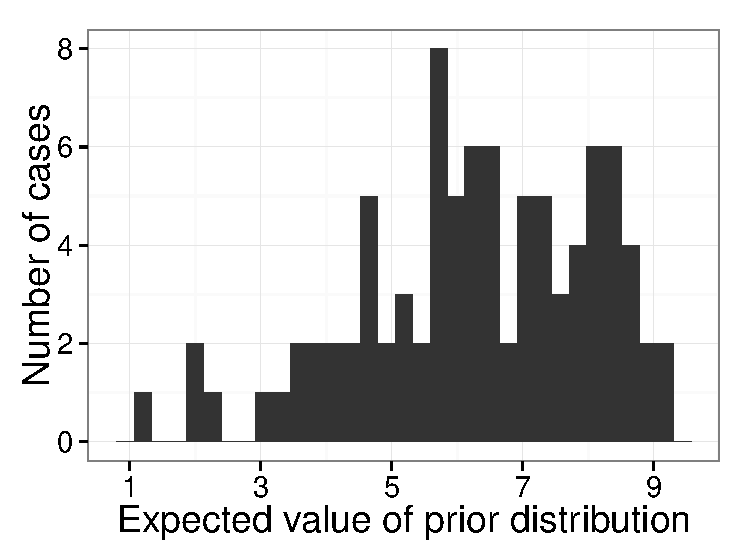
\includegraphics[width=.5\textwidth]{pics/priorexpectations-histogram}	
	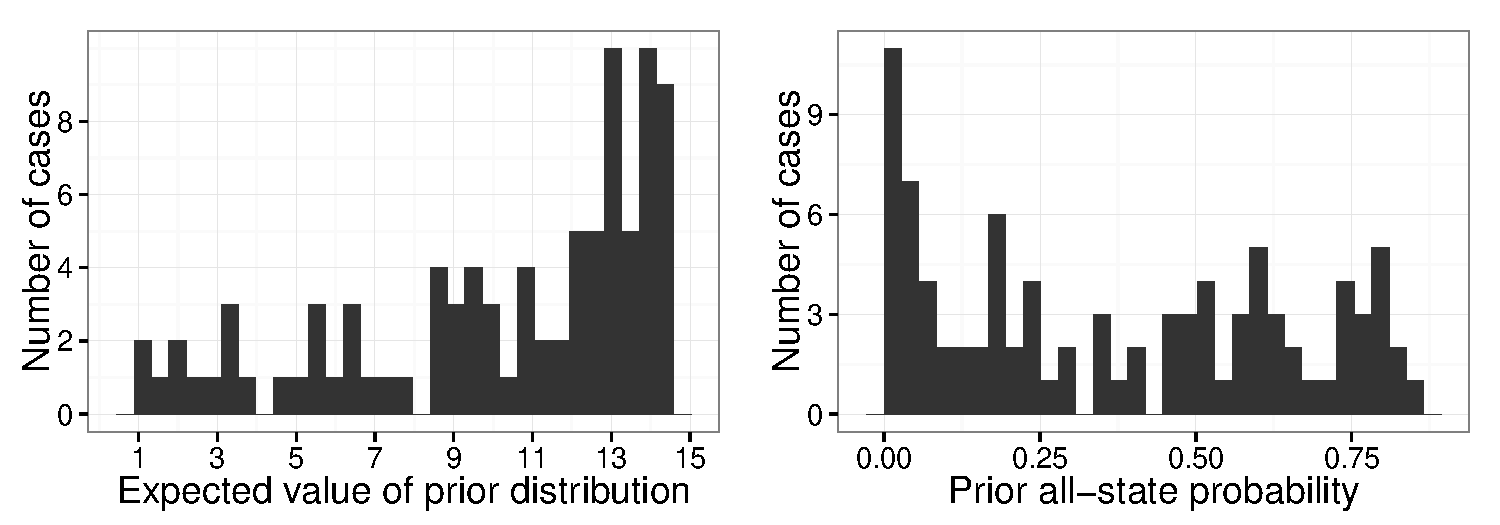
\includegraphics[width=.9\textwidth]{pics/priordistributions}	
	\caption{Histogram of expected values $\mathbb{E}[P(s)]$ of each empirically elicited and smoothed prior distribution (left) and histogram of prior probabilities $P(s_{15})$  of the all-state for each item (right).}
	\label{fig:probhist}	
\end{figure}

In the next section, we use the underlying prior beliefs inferred from the two different dependent measures to derive RSA predictions for the interpretation of utterances like \emph{Some of the marbles sank}, before empirically measuring participants' interpretations.



\section{Effect of the world prior in RSA}
\label{sec:rsa}

The basic Rational Speech Acts model defines a pragmatic listener $P_{L_1}(s|u)$ who reasons about a speaker $P_{S_1}(u|s)$, who in turn reasons about a literal listener $P_{L_0}(s|u)$. Each listener performs Bayesian inference about the world state the speaker intends to communicate, given either the literal truth of utterance $u$ or the speaker's choice of $u$; the speaker is a softmax-optimal decision maker, with the goal of being informative about the state $s$.
RSA is defined by: 
\begin{eqnarray}
&&P_{L_0}(s|u)\propto \delta_{\denote{u}(s)} \cdot P(s)\\
&&P_{S_1}(u|s) \propto \mathrm{exp}({\lambda \ln P_{L_0}(s|u))}\\ 
&&P_{L_1}(s|u)\propto P_{S_1}(u|s)\cdot P(s)
\end{eqnarray}
Here $\denote{u}: S \rightarrow \text{Boolean}$ is a truth-function specifying the literal meaning of each utterance and $\delta_{\denote{u}(s)}$ is the Kronecker delta function returning a uniform distribution over all states $s$ compatible with utterance $u$.

For concreteness, assume that the set of states of the world is $S = \{s_0, s_1, s_2, \dots, s_{15}\}$, where the subscript indicates the number of objects (e.g., marbles) that exhibit an effect (e.g., sinking). 
Further assume that the set of three utterances \emph{All/None/Some of the marbles sank} is denoted $U = \{u_{\textrm{all}}, u_{\textrm{none}}, u_{\textrm{some}}\}$ and each has its usual literal meaning: 
%$\denote{u_{\textrm{none}}}: s=0$,  
%$\denote{u_{\textrm{some}}}: s>0$,
%$\denote{u_{\textrm{all}}}: s=15$.
$\denote{u_{\textrm{none}}}= \{s_i | i = 0\}$,  
$\denote{u_{\textrm{some}}}= \{s_i | i > 0\}$,
$\denote{u_{\textrm{all}}}= \{s_i | i = 15\}$.

%Let us imagine that the prior is binomial with single event probability $\theta$: $P(s)=\text{Binomial}(s|\theta)$.

\begin{figure*}
	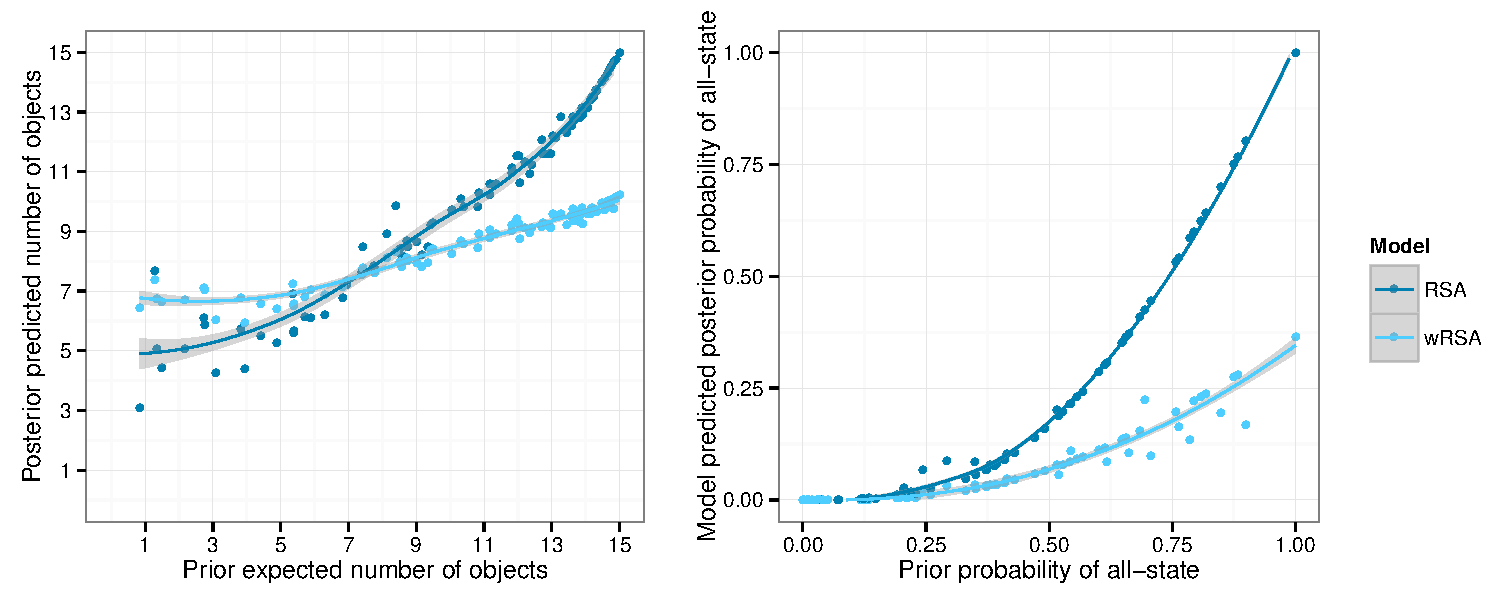
\includegraphics[width=\textwidth]{pics/rsa-predictions}
%	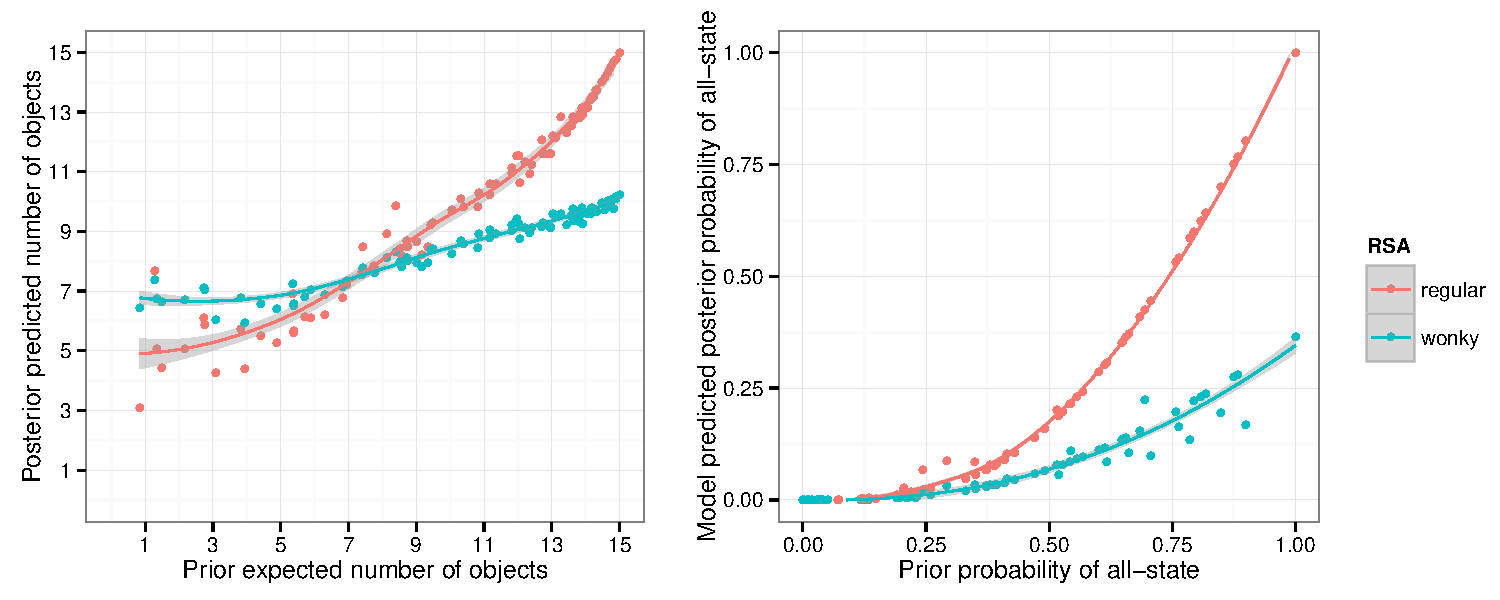
\includegraphics[width=\textwidth]{pics/rsa-predictions-uniform}	
	\caption{For each item, RSA and wRSA model predicted $\mathbb{E}[P(s|u_{\textrm{some}})]$ as a function of $\mathbb{E}[P(s)]$ (left) and $P(s_{15}|u_{\textrm{some}})$ as a function of $P(s_{15})$ (right).}
	\label{fig:rrsaexppredictions}	
\end{figure*}

In Figure \ref{fig:rrsaexppredictions} we show the predictions of RSA (dark blue dots) for the items from Exps.~1a and 1b in two different ways: the left panel shows the posterior expected number of affected objects as a function of the prior expectation; the right panel shows the posterior probability of the state in which all objects are affected, as a function of the prior probability of that state.\footnote{That the individual model predictions look somewhat noisy is due to the different shapes of the prior distributions, such that for the same expected value of the distribution, the distribution itself can take different shapes, which are treated slightly differently by the model.}   %as $\theta$ varies. \red{put in figure showing the basic RSA predictions for allstate $P(s_{15}|u_{some})$ and expectation. this figure could also have wRSA predictions for later reference.} 
We see that the prior has a strong effect, which can be summarized by the two predictions described in the Introduction: 
\begin{enumerate}
	\item $P(s_{15}|u_{\textrm{some}}) \rightarrow 1$ as $P(s_{15})\rightarrow 1$
	\item $\mathbb{E}[P(s|u_{\textrm{some}})] \simeq \mathbb{E}[P(s)]$ over the upper half of its range. 
\end{enumerate}
We next turn to an empirical test of these predictions, or rather, of the intuition that they may be incorrect.

%\section{Models of utterance interpretation}
%
%
%Recent Bayesian Rational Speech Act (RSA)  \cite{frank2012} and game-theoretic \cite{franke2011} models that treat communication as a signaling game \cite{lewis} between a speaker and a listener have successfully captured listeners' quantitative  behavior on a number of pragmatic inference tasks, including ad hoc Quantity implicature \red{ref}, M-implicature \red{ref}, scalar implicature \red{ref}, and embedded scalar implicatures \red{ref}. In these models, the listener reasons about likely utterances a speaker will produce who is trying to be informative with respect to a na\"ive listener. These models make clear predictions about how prior beliefs about states of the world should be integrated with listeners' expectations about utterances a speaker is likely to produce to communicate a particular state of the world. 
%
%\red{i think we should hold the math for the model section. it doesn't really add much here... without it, this section can be folded nicely into the introduction.}
%
%For concreteness, assume that $S = \{s_0, s_1, s_2, \dots, s_{15}\}$ is the set of states of the world, where the subscript indicates the number of objects (e.g., marbles) that exhibit a certain effect (e.g., sinking). Assume further that $U = \{u_{\textrm{all}}, u_{\textrm{none}}, u_{\textrm{some}}\}$, the set of utterances \emph{All/None/Some of the marbles sank}. The speaker chooses an utterance to convey $s$ proportional to the soft-max expected utility of producing $u$ to communicate $s$, where utility is determined by how uncertain a listener remains: \red{what's the expectation doing?}
%
%\begin{equation}
%P_{S_1}(u|s) \propto \mathrm{exp}({\lambda \mathbb{E} (\ln P_{\textrm{lex}}(s|u))})
%\end{equation}
%
%where $P_{\textrm{lex}}(s|u)$ is the literal interpretation probability resulting from each utterance's truth-functional meaning: $F_u: s \mapsto \{0,1\}$. \red{need to spell out lit listener since the prior enters there too} The listener's task is to infer a distribution over $S$, given an utterance $u$ produced by the above defined informative speaker. %$p(s|u)$, that is, the probability of the state of the world the speaker intended to communicate (e.g., how many friends came to a party), given that the speaker produced $u$ (e.g., \emph{some of my friends came to the party}). 
%By Bayes' rule: 
%\begin{equation}
%P_{L_1}(s|u)\propto P_{S_1}(u|s)\cdot P(s)
%\end{equation}
%That is, the inferred listener probabilities are proportional to the product of both the speaker's utterance probabilities and the listener's prior beliefs in different numbers of marbles sinking. Using a uniform prior over the state space, this model has been very successful at capturing \emph{scalar implicatures} \cite{grice1975}. These are inferences that arise in cases of utterances like \textit{Some of the marbles sank}, which typically give rise to the inference that not all of the marbles sank. Scalar implicatures fall out of the fact that the speaker probability of producing $u_{\textrm{some}}$ in $s_{15}$ is low (because there is an alternative utterance $u_{\textrm{all}}$ which has a higher probability of being used for $s_{15}$ because it is more informative about that state). However, the role of prior beliefs in RSA models remains under-explored, both with respect to scalar implicature computation as well as with respect to utterance interpretation more generally.
%
%
%%One important consequence of the standard RSA model is that the listener's prior beliefs will not affect the interpretation of $u$ very strongly, if at all,  where the semantics of $u$ is highly constraining, that is, where  $P_{\textrm{lex}}(s|u)$ is very peaked. For example, an utterance of \emph{All of the marbles sank} is highly constraining because all of the probability mass ends up on $s_{15}$ by virtue of the semantics of $u_{\textrm{all}}$ alone, regardless of how likely the listener believes marbles sink a priori.\footnote{We ignore hyperbolic interpretations of universal quantifiers here.} 
%
%One important consequence of the standard RSA model is that where the semantics of $u$ is weak---that is, where $F_u$ accepts many states---prior beliefs are predicted to have a large effect on the resulting listener belief distribution. For example, an utterance of \emph{Some of the marbles sank}, produced in a situation in which any of 0 - 15 of 15 contextually established marbles could have sunk, semantically only restricts the state space by one state (that in which 0 marbles sank). In this case, listeners' prior beliefs about sinking marbles will have a large effect on their posterior belief distribution. If the listener believes that marbles rarely sink, the utterance will be interpreted as conveying that fewer marbles sank than if the listener believes marbles almost always sink. The predictions this model makes for the interpretation of $u_{\textrm{some}}$ -- both for $P_{L_1}(s_{15}|u_{\textrm{some}})$ and for the expected value of $P_{L_1}(s|u_{\textrm{some}})$ as a function of $P(s_{15})$ and the expected value of $P(s)$, respectively  -- are shown in \figref{fig:rrsaexppredictions}. RSA predicts that the probability of the state in which all objects exhibit a certain effect increases with increasing $P(s_{15})$, such that for $P(s_{15})$ close to 1, $P_{L_1}(s_{15}|u_{\textrm{some}})$ approaches 1. Relatedly, with increasing expected value of the prior belief distribution $P(s)$, so is the expected value of the posterior belief distribution predicted to increase, approaching 1). \red{hmm... i think we either need to focus on the allstate probs for this motivation, or already point to the data from expt 1.}
%
%However, intuition is at odds with this prediction: for example,  \citeA{geurts2010} has observed that for events with very high prior probability of occurrence (e.g.~marbles sinking), observing an utterance of \emph{Some of the marbles sank} leads to very strong implicatures, that is, the subjective probability  that not all of the marbles sank is intuitively close to 0. Given the previous success of RSA models, this constitutes a striking puzzle, and one we set out to solve here. In doing so, we pursue the intuition raised at the very beginning of this paper: that sometimes, the speaker's utterance will lead the listener to infer that the world under discussion is wonky and she should therefore down-weight her prior beliefs in the computation of speaker meaning.
%
%
%Our contribution is two-fold: first, we collect empirical estimates of $P(s)$ and $P_{L_1}(s|u)$ to investigate the empirical effect of listeners' prior beliefs on interpretation. Second, we extend the RSA model to incorporate a free variable $\theta_{\textrm{wonky}}$ that captures the extent to which the listener believes the described event is wonky  and she should thus discount her prior beliefs when interpreting $u$. We refer to this model as \emph{wonky RSA (wRSA)} in contrast to \emph{regular RSA (rRSA)}. Wonkiness inferences in wRSA are triggered by the surprisal of a produced utterance $u$, given listeners' prior beliefs, capturing that listeners expect speakers' utterances to be both truthful and informative with respect to prior beliefs. To the extent that they are not, listeners will have to either infer that the speaker is being uncooperative, or else assume that they may need to revise their beliefs about the world. Here we pursue the latter possibility.
%
%This paper is structured as follows. We first report the results of three experiments (1, 2a, 2b) that show that while there is an effect of the prior on listeners' interpretations of sentences like \emph{Some of the marbles sank}, this effect is much smaller than predicted by rRSA. Exp.~3 provides evidence that listeners' beliefs about object or event wonkiness are indeed influenced by the surprisal of the utterance. Finally, we present wRSA as an extension of rRSA that incorporates the idea of backing off to alternate prior beliefs if the observed utterance suggests a wonky world. This model provides a much better fit to the empirical data from Exps.~2a and 2b than rRSA, and also provides a good fit to the wonkiness ratings obtained in Exp.~3.




\section{Experiment 2a and 2b: comprehension}  
\label{sec:comprehension}

Exps.~2a and 2b\footnote{These experiments can be viewed at \url{http://cocolab.stanford.edu/cogsci2015/wonky/expectation/sinking-marbles.html} and \url{http://cocolab.stanford.edu/cogsci2015/wonky/stateprobs/sinking-marbles-nullutterance.html}}  measured participants' posterior beliefs $P(s|u)$ about how many objects exhibited a certain effect (e.g., marbles sinking), after observing an utterance. The only difference between the experiments was the dependent measure. The dependent measures differed in order to directly and independently estimate the two values that the  predictions above are concerned with: $\mathbb{E}[P(s|u_{\textrm{some}})]$ and $P(s_{15}|u_{\textrm{some}})$, i.e., the expected number of X that are deemed to have Yed and the probability of all of the X having Yed (a measure of implicature strength), respectively, after observing the utterance \emph{Some of the X Yed}.

\subsection{Method}

\subsubsection{Participants}
For each experiment we recruited 120 participants over Amazon's Mechanical Turk who were paid \$0.70  for their participation.

\subsubsection{Procedure and materials}

Participants read the same descriptions as in Exps.~1a and 1b. They additionally saw an utterance produced by a knowledgeable speaker about the event, e.g.~\textit{John, who observed what happened, said: ``Some of the marbles sank''}. In Exp.~2a (just as in Exp.~1a), they then provided a judgment of an effect, e.g.~\textit{How many of the marbles do you think sank?}, on a sliding scale from 0 to 15. In Exp.~2b they instead rated on sliding scales with endpoints labeled ``definitely not'' and ``definitely'', how likely they thought 0\%, 1-50\%, 51-99\%, or 100\% of the objects exhibited the effect.

Each participant saw 10 \emph{some} trials and 20 filler trials, of which 10 contained the quantifiers \emph{all} or \emph{none}, and the rest were utterances that did not address the number of objects that displayed the effect. These 10 additional fillers were intended to establish a baseline for participants' use of information about the prior. Of these, half were generic short fillers that were intended to communicate the prior, e.g., \emph{Typical}. The rest were longer sentences that addressed a different aspect of the described scenario, e.g.~\emph{What a stupid thing to do}.\footnote{See \appref{sec:items} for a complete list of items.} The utterances were randomly paired with 30 random items for each participant.

 
\begin{figure*}
	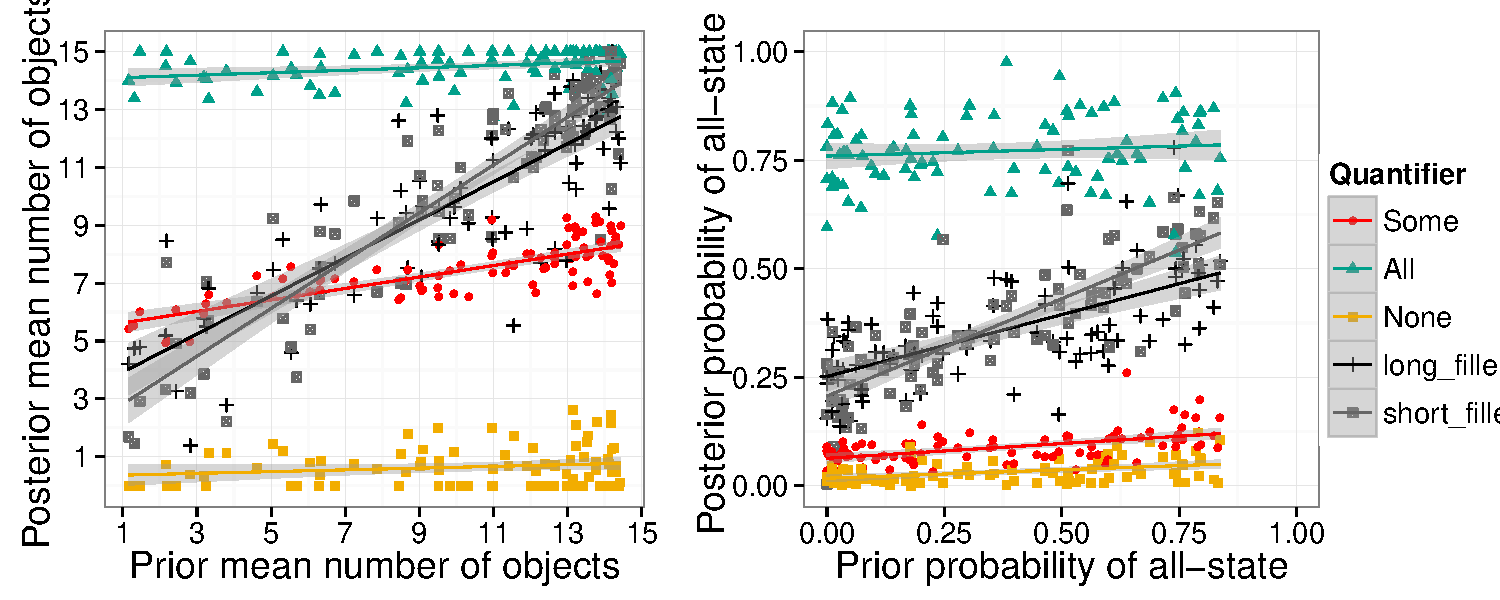
\includegraphics[width=\textwidth]{pics/empirical-results}	
	\caption{For each item and quantifier, empirical $\mathbb{E}[P(s|u_{\textrm{some}})]$ from Exp.~2a against $\mathbb{E}[P(s)]$ from Exp.~1 (left)  and empirical $P(s_{15}|u_{\textrm{some}})$ from Exp.~2b against  $P(s_{15})$ from Exp.~1 (right).}
	\label{fig:empiricalresults}	
\end{figure*}

 
 \subsection{Results and discussion}

Data from Exp.~2a were analyzed as given. Slider ratings obtained in Exp.~2b were first subjected to normalization on a by-trial and by-participant basis, such that on each trial, a participant's ratings added to 1, i.e., constituted a proper probability distribution. After normalization, data from eight participants in Exp.~2b were excluded from the analysis because these participants assigned less than 0.8 probability to the interpretation corresponding to the correct literal interpretation on literal \emph{all} and \emph{none} trials.\footnote{In general, this task yielded noisier results than the task in Exp.~2a (as can be seen in the average lower probability of the all- state after observing \emph{all}, in the right panel of \figref{fig:empiricalresults}) because participants used the sliders in different ways. For example, for cases where intuitively, the all-state was true, some participants assigned non-zero probability to only the all-state, while others were reluctant to do so and always assigned some probability to the 51-99\% state.}

The main question of interest was whether the predictions of the basic RSA model laid out in the previous section were borne out in participants' judgments of how many X Yed after hearing an utterance with \emph{some}. Mean empirical $\mathbb{E}[P(s|u)]$ (expected value of the posterior distribution) and $P(s_{15}|u)$ (posterior all-state probability) are shown in \figref{fig:empiricalresults} for each item. Visual inspection of the graphs shows that the interpretation of utterances with \emph{all} and \emph{none} seems to be relatively unaffected by the prior, while the interpretation of \emph{some} displays a small, but robust, effect. 

To test whether the visual effect of the prior on the interpretation of \emph{some} is real, we conducted linear mixed effects regressions on the \emph{some} data from each experiment. For Exp.~2a, the number of X that Yed  was regressed onto centered fixed effects of each item's prior expectation and trial number (to account for changes in response behavior over the course of the experiment). For Exp.~2b, the  all-state probability was regressed onto centered fixed effects of each item's prior all-state probability and trial number. Each model also contained the maximal by-item and by-participant random effects structure, following the guidelines outlined by \citeA{barr2013}. \red{Rerun all the analyses once you get numbers from MH.}    

For utterances of \emph{Some of the X Yed}, the mean number of objects judged to exhibit the effect increased with increasing expectation of the prior distribution ($\beta$=.18, $SE$=.02, $t$=7.4, $p$$<$.0001). Similarly, the probability of all 15 objects exhibiting the effect increased with increasing prior probability of doing so ($\beta$=.06, $SE$=.01, $t$=5.0, $p$$<$.0001). However, the size of these effects is, to say the least, much smaller than predicted by RSA (for comparison, see dark lines in \figref{fig:rrsaexppredictions}).

One possible explanation for this highly attenuated effect of the prior is that participants simply did not bring world knowledge to bear on the interpretation of utterances. However, this possibility is ruled out by examining participants' performance in the filler conditions: in both Exps.~2a and 2b, the filler conditions closely tracked the prior (see \figref{fig:empiricalresults}). Additionally, that there is any effect of the prior at all suggests that participants are not entirely disregarding their prior beliefs.

Exps.~2a and 2b thus demonstrate that there is an effect of listeners' prior beliefs on the interpretation of utterances with \emph{some}. However, this effect is quantitatively much smaller than predicted by RSA, and qualitatively does not match the predictions identified above: the implicature is not canceled for extreme priors (contra prediction (1)) and the posterior expectation diverges from the prior expectation (contra prediction (2)).
In the next section, we extend the RSA model to formalize the intuition, raised in the Introduction, that a listener may decide that her initial beliefs about the domain are not shared by the speaker and respond by revising her priors.


\section{Effect of the world prior in `wonky RSA'}
\label{sec:wrsa}

To capture the idea that the pragmatic listener is unsure what background knowledge the speaker is bringing to the conversation, we extend the basic RSA model by using a ``lifted variable''  \cite{goodmanlassiter,lassiter2013,bergengoodman2012,kao2014} corresponding to the choice of state prior. A lifted variable is a variable that the model (in particular, the pragmatic listener) reasons about explicitly instead of being given a value for it. In this case, we posit that the prior, now $P(s|w)$, depends on a ``wonkiness'' variable $w$, which determines whether to use the ``usual'' prior for this domain or a more generic back-off prior, which we take to be uniform:\footnote{\red{a footnote either briefly discussing other priors or delaying such a discussion to the general discussion}}
$$
P(s|w) \propto \begin{cases}
1  & \text{if } w\\
   P_{\text{usual}}(s) & \text{if not } w
  \end{cases}
  $$
  
This inferred prior is used in both the literal and pragmatic listeners, indicating that it is taken to be common ground. However, the $w$ variable is reasoned about only by the pragmatic listener, which captures the idea that it is an inference the pragmatic listener makes about which assumptions are appropriate to the conversation. Using the notation of \sectionref{sec:rsa}:
\begin{eqnarray}
&&P_{L_0}(s|u,w)\propto \delta_{\denote{u}(s)} \cdot P(s|w)\\
&&P_{S_1}(u|s,w) \propto \mathrm{exp}({\lambda \ln P_{L_0}(s|u,w))}\\
&&P_{L_1}(s,w|u)\propto P_{S_1}(u|s,w)\cdot P(s|w) \cdot P(w)
\end{eqnarray}
We refer to this model as wRSA. Notice that the choice of $w$ that the listener makes will depend on $P_{S_1}(u|s,w)$: if a given utterance can't be explained by the usual prior, because it is unlikely under any plausible world state $s$, then the pragmatic listener will infer that the world is wonky, and back off to the uniform prior.
That is, if the utterance is odd, the listener will revise her opinion about what world knowledge is appropriate to use. \red{we need to explain where oddness comes from -- maybe there's an easy graphical way of showing how for items with different priors, a `some' utterance is more or less wonky, by showing the marginal probabilities of observing each utterance for these different items?}

\red{update this bit with mh's numbers} To make predictions for Exps.~2 from wRSA we use the inferred priors from Exps.~1 as $P_{\text{usual}}(s)$ for each item. The wonkiness prior $P(w)$ and the speaker optimality parameter $\lambda$ are fit to optimize mean squared error (MSE) with Exp.~2 data. The optimal parameters ($\lambda = 2$, $P(w) = 0.5$) resulted in an MSE of 2.15 (compared to 14.53 for RSA) for the expected number of objects, and 0.01 (compared to 0.07 for RSA) for the all-state probability. The better fit of wRSA compared to RSA can be seen in the comparison of \figref{fig:rrsaexppredictions} and \figref{fig:empiricalresults}: in both cases, wRSA (light blue lines) predicts a much attenuated effect of the prior compared to regular RSA (dark blue lines), in line with the empirical data. Furthermore, wRSA does not make either of the problematic predictions identified earlier for regular RSA.% (i.e., suspension of the implicature under high all-state probabilities and tracking of the expected value of the prior distribution in the upper range).


These results are encouraging: wRSA is able to account for the qualitative and quantitative departures of participants' behavior from RSA, with respect to the effect of the prior.
Is this because listeners are actually inferring that the world is unusual from an utterance like \emph{Some of the marbles sank}?
The wRSA model makes predictions about the probability that a given world is wonky after observing an utterance; see the left panel of \figref{fig:wonkymodel} for predicted wonkiness probabilities for $u_{\textrm{all}}$, $u_{\textrm{none}}$, and $u_{\textrm{some}}$ using the  optimal $P(w)$ and $\lambda$ parameters from fitting wRSA to the Exp.~2 data.
Note the U-shaped curve, in which the world is judged wonky if $u_{\textrm{some}}$ is used in worlds with extreme priors.
 We can test these predictions directly by simply asking participants for each item from Exps.~2a and 2b, whether they believe the described situation is normal.



\begin{figure}
%	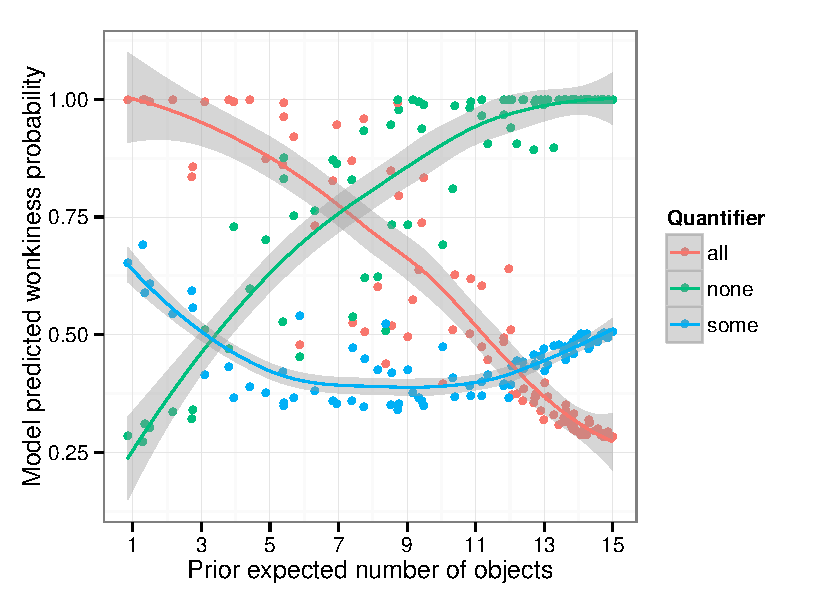
\includegraphics[width=.5\textwidth]{pics/model-wonkiness-binomial}
%	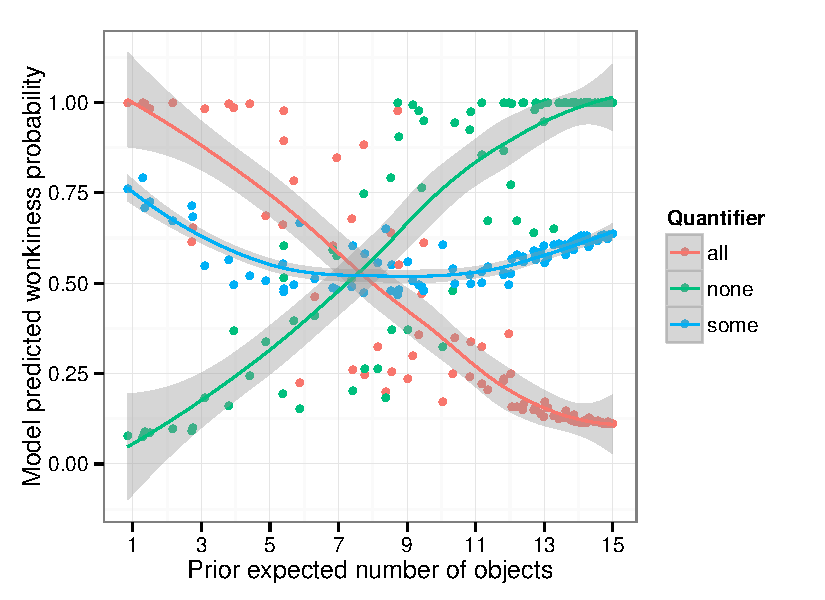
\includegraphics[width=.5\textwidth]{pics/model-wonkiness-uniform}
	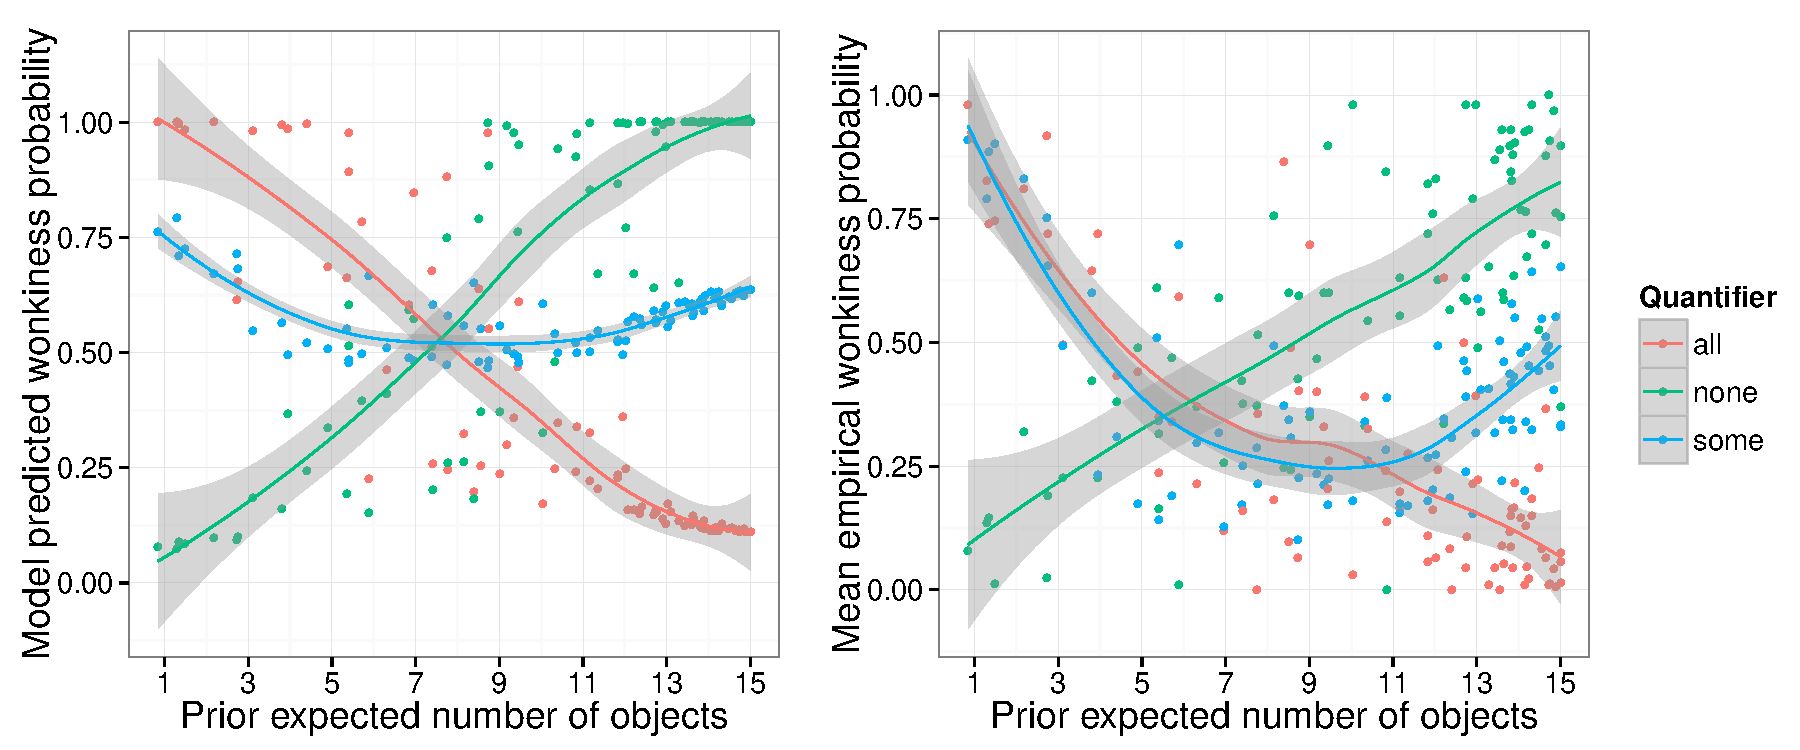
\includegraphics[width=.9\textwidth]{pics/wonkiness-fullplot}
	\caption{For each item, predicted (left) and empirical (right) wonkiness probability after observing an utterance ($u_{\textrm{all}}, u_{\textrm{none}}, u_{\textrm{some}}$), as a function of the prior expected number of affected objects.}
	\label{fig:wonkymodel}	
\end{figure}

\section{Experiment 3: wonkiness}
\label{sec:wonkiness}

Exp.~3\footnote{This experiment can be viewed at \url{http://cocolab.stanford.edu/cogsci2015/wonky/wonkiness/sinking-marbles-normal.html}} measured participants' beliefs in world wonkiness after observing the scenarios and utterances from Exps.~2a and 2b.

\subsection{Methods}

\subsubsection{Participants}
We recruited 60 participants over Amazon's crowd-sourcing platform Mechanical Turk who were paid \$0.50  for their participation.

\subsubsection{Procedure and materials}

The procedure and materials were identical to those of Exps.~2a and 2b, with the exception of the dependent measure. Rather than providing estimates of how many X they believed Yed, participants were asked to indicate how likely it was that the objects  (e.g., the marbles) involved in the scenario were normal objects, by adjusting a slider with endpoints labeled ``definitely not normal'' to ``definitely normal.''

\subsection{Results and discussion}

The extreme ends of the sliders were coded as 1 (``definitely not normal'', i.e., wonky) and 0 (``definitely normal'', i.e., not wonky). We interpret the slider values as probability of world wonkiness. Mean wonkiness probability ratings are shown in the right panel of \figref{fig:wonkymodel} and closely mimic wRSA's predictions (see left panel of \figref{fig:wonkymodel}). For $u_{\textrm{all}}$ and $u_{\textrm{none}}$, increasing prior expectation of Xs Ying resulted in a fairly linear decrease and increase in the probability of wonkiness, respectively. For $u_{\textrm{some}}$, the pattern is somewhat more intricate: probability of wonkiness initially decreases sharply, but rises again in the upper range of the prior expected value. 
%
%\begin{figure}
%	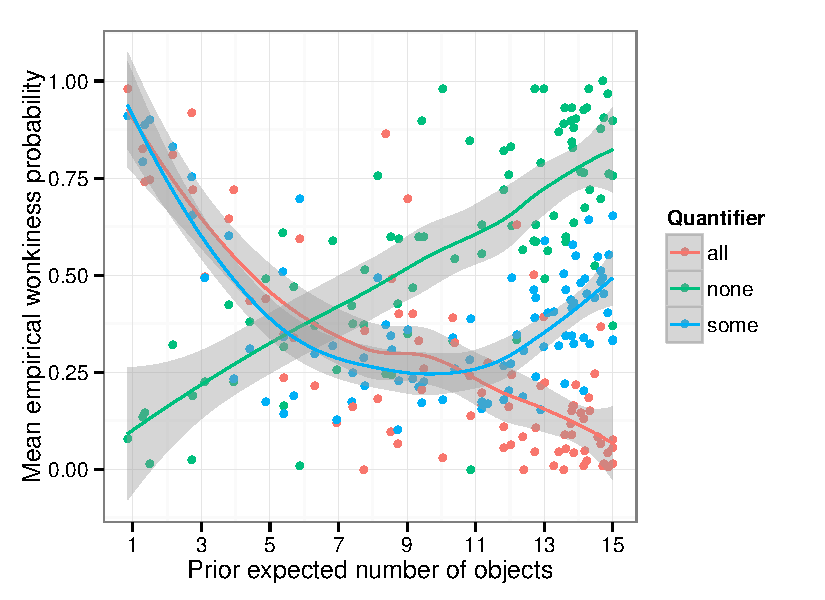
\includegraphics[width=.5\textwidth]{pics/empirical-wonkiness}
%	\caption{For each item, mean empirical wonkiness probability after observing an utterance ($u_{\textrm{all}}, u_{\textrm{none}}, u_{\textrm{some}}$), as a function of the prior expected  number of affected objects.}
%	\label{fig:wonkyratings}	
%\end{figure}

Qualitatively, the model captures both the linear increase and decrease in wonkiness probability for $u_{\textrm{all}}$ and $u_{\textrm{none}}$, respectively. Importantly, it also captures the asymmetric U-shaped wonkiness probability curve displayed by $u_{\textrm{some}}$. Intuitively, this shape can be explained as follows: for very low probability events, it is surprising to learn that such an event took place (which is what is communicated by $u_{\textrm{some}}$), so wonkiness is high. For medium probability events, learning that this event took place is not very surprising, so wonkiness is relatively low. For high probability events, $u_{\textrm{some}}$ may be literally true, but it is not useful in the sense of providing the listener new information. For comparison to the comprehension data fit, the model's MSE for empirical wonkiness probability predictions, using the best parameters from fitting the model to the comprehension data, was 0.07. 

That the wonkiness probability predictions are borne out in the empirical data provide further support for wRSA, and for the idea that participants are revising their prior beliefs online when encountering an odd utterance. \red{put in here somewhere the relation between wonkiness and the comprehension data: for all and none, while there are huge changes in wonkiness by prior, we don't expect this to show up in the comprehension data because the semantics of the utterances restricts the interpretation to just one state, regardless of the prior. but for "some", which has a weak semantics, wonkiness shifts the overall interpretation in a way that compresses the effect of the prior}


Some readers may still not be convinced that what is driving the attenuated effect of the prior is that listeners revise their beliefs about the world (or about the event, or the objects involved in the event---we return to this issue in the general discussion). A prima facie alternative possibility to why prior beliefs have a much smaller effect than expected on utterance interpretation is that listeners believe that the speaker is an unreliable or uncooperative speaker, one who talks about the world in surprising and unexpected ways. For example, maybe participants in the studies reported thus far believed that the speaker was a) lying, b) not trying to be informative, c) or not actually knowledgeable about the precise state of the world, i.e., about how many X Yed.

There are multiple reasons why this is not a plausible explanation for our results. First, participants were happy to interpret the speaker's utterances literally in the \emph{all} and \emph{none} conditions, suggesting they didn't believe the speaker was lying, ruling out a). Second, the wonkiness judgments obtained in Exp.~3 closely match the wRSA model's predictions, which relies on speaker reliability and cooperativity---knowing the actual state of the world and reporting it truthfully and informatively---, ruling out b) and c). However, there is an even clearer reason for ruling out speaker reliability explanations for the observed attenuated effect of the prior: if the speaker was actually unreliable, intuition and the (RSA and wRSA \red{make sure this is actually true for both and see if there are note-worthy differences}) model predict that listeners should use their prior world knowledge much more strongly than if the speaker was reliable. For example, if my very successful but understated friend says that he did ``OK'' on a job interview, I'll be more likely to disregard his pronouncement of mediocre performance and expect him to have done very well. That is, speaker unreliability predicts a much greater effect of the prior on interpretation than we observe empirically. 

\red{To see this from the model's perspective, XXX discuss effect of setting lambda to 0: random choice between between true utterances) put actual model predictions in a plot}


These considerations make the following prediction: if speaker reliability is explicitly manipulated, listeners' interpretations of \emph{Some of the X Yed} should be much more strongly governed by their prior beliefs when the speaker is unreliable/uncooperative than when the speaker is reliable/cooperative. That is, we expect a replication of Exp.~2b for reliable, but not unreliable speakers. If, instead, there is something more fundamentally wrong with RSA models and the attenuated effect of the prior on comprehension is driven by listeners' perception of the speaker as unreliable, further decreasing speaker reliability should have no effect on how strongly the prior influences listeners' interpretations. If anything, explicitly unreliable speakers should further diminish the effect of the prior. We test the prediction about speaker reliability in Exp.~4.

\section{Exp.~4: speaker reliability}
\label{sec:speakerreliability}

Exp.~4\footnote{This experiment can be viewed at \url{http://cocolab.stanford.edu/cogsci2015/wonky/speakerreliability/sinking-marbles.html}.} explores how speaker reliability interacts with prior beliefs in the interpretation of the same utterances as in Exps.~1-3. As discussed in the previous section, the wRSA model predicts that listeners' interpretation of \emph{Some of the X Yed} should be more strongly affected by their prior beliefs when the speaker is perceived as unreliable than when the speaker is perceived as reliable. There are different ways in which speaker reliability can be construed. Here, we are interested in manipulating speaker reliability in such a way as to lead listeners to expect underinformativity or truthful (but wrong) reports of misperceived events. To this end, we introduce two unreliable speakers: a speaker who has an incentive to be misleading in a courtroom scenario and a drunk speaker. These speakers are contrasted within participants with a reliable speaker.

Exp.~4 was very similar to Exp.~2b, but used only half of the items and a blocked design. In each block, the speaker who described observed events remained the same throughout the block. The speaker's reliability was established via a short cover story at the beginning of each block. This allowed us to compare the effect of prior beliefs on participants' interpretations of \emph{Some of the X Yed} uttered by speakers of differing reliability.

\subsection{Method}

\subsubsection{Participants}

We recruited 120 participants over Amazon's Mechanical Turk who were paid \$1.00 for their participation. 

\subsubsection{Procedure and materials}

Participants were first introduced to a party scenario with three (randomly generated) characters, here James, Emily, and Robert:

\begin{quote}
Yesterday, James, Emily, and Robert went to a big, crazy party that lasted all day. Everyone was playing games and having fun. In this study, you'll read about James, Emily, and Robert's experiences at the party and answer simple questions.
\end{quote}

They then proceeded through three blocks of fifteen trials each, for a total of 45 trials. On each block, one of the three characters introduced initially was the speaker. Speaker reliability was manipulated via a short description of the speaker at the beginning of each block. One speaker was reliable (\emph{sober} condition) and two were unreliable (\emph{drunk} and \emph{court} condition). Block order was randomized.  The following are examples of speaker descriptions for the block order \emph{sober - drunk - court}.

\emph{Sober:}
\begin{quote}
Flashback to the party: James likes to comment on events he observes. He also likes to keep a clear mind, so he is staying sober. He's having a great time going around observing what people are doing and commenting on what happens.
\end{quote}

\emph{Drunk:}
\begin{quote}
Now you know how James experienced the party. Next up is Emily.

Flashback to the party: Emily is pretty drunk. Her speech is slurred. At one point she thinks she sees a flying pig. But she's having a great time going around observing what people are doing. She describes what happens to anyone who will listen.
\end{quote}

\emph{Court:}
\begin{quote}
Now you know how Emily experienced the party, too. Next up is Robert.

It's the day after the party. Robert has been asked to appear in court. He was witness to events at the party that resulted in damaged property. The prosecutor asks him questions about the events that transpired. In each case, John saw exactly what happened. But he also wants to protect his friends.
\end{quote}

\begin{table}
\caption{Overview of trial structure in the different blocks (\emph{sober, drunk, court}) of Exp.~4.}
\begin{tabular}{l p{4.2cm} p{4.2cm} p{4.2cm}}
\toprule
 & \centering \emph{sober} & \centering \emph{drunk} & \centering \emph{court} \tabularnewline
\midrule
Event & \multicolumn{2}{c}{At the party, Diane threw 15 marbles into the pool.} & The prosecutor says: ``Diane threw 15 marbles into the pool. What happened next?''\\
\midrule
Speaker & James, who interestedly observed what happened, says, & Emily, who drunkenly observed what happened, says, & Robert, who observed what happened but wants to protect his friends, says,\\
\midrule
Utterance & \multicolumn{3}{c}{``Some of the marbles sank.''}\\
\midrule
Question & \multicolumn{3}{c}{How many marbles sank?}\\
\bottomrule
\end{tabular}
\label{tab:trialstructure}
\end{table}

On each trial, participants performed the same task as in Exp.~2b: they saw a sentence introducing an event (e.g., \emph{At the party, Diane threw 15 marbles into the pool}), followed by a sentence about the speaker (e.g., \emph{James, who interestedly observed what happened, says,}), followed by the speaker's utterance (e.g., \emph{``Some of the marbles sank''}). They were then asked to rate on four sliding scales with endpoints labeled ``definitely not'' and ``definitely'', how likely they thought 0\%, 1-50\%, 51-99\%, or 100\% of the objects (e.g., marbles) exhibited the effect (e.g., sank). The different speaker scenarios made it impossible to maintain an identical trial structure across blocks, but we attempted to minimize the differences in trial structure across blocks, while including material that reminded participants about the speaker's situation. See \tableref{tab:trialstructure} for an overview of trial structure in each block.

In Exp.~4, only half of the items from Exps.~1-3 were used; those 45 that described events that could plausibly have occurred at a day-long party, while nevertheless spanning the entire range of prior probabilities. See \appref{sec:items} for the full list of items. Each block contained the same distribution of utterances: two \emph{all} trials, two \emph{none} trials, two short filler trials, two long filler trials, and seven \emph{some} trials. Items were distributed over utterances so that each participant saw each item once, i.e., no participant saw for example the \emph{sinking marbles} item with both the \emph{some} and the \emph{all} utterance.

\subsection{Results and discussion}

\begin{figure}
	\centering
	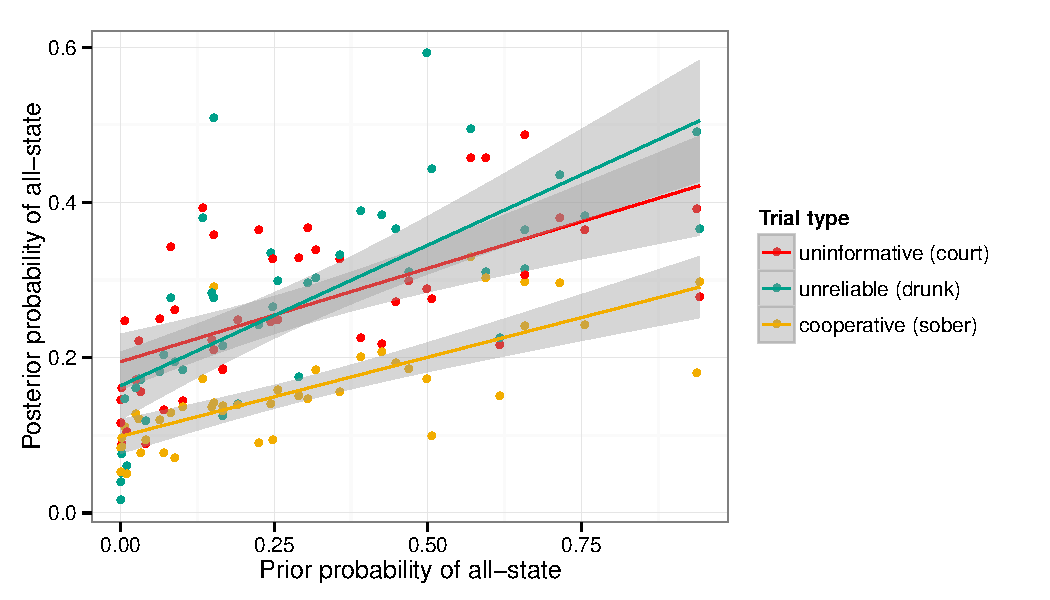
\includegraphics[width=.6\textwidth]{pics/speakerreliabilityresults}
	\caption{For each item, empirical mean posterior $P(s_{15}|u_{\textrm{some}})$ against  prior $P(s_{15})$ from Exp.~1, separately for reliable (\emph{sober}) and unreliable (\emph{drunk, court}) speakers.}
	\label{fig:speakerreliability}	
\end{figure}

Mean posterior $P(s_{15}|u_{\textrm{some}})$ ratings for the different speaker reliability conditions are shown in \figref{fig:speakerreliability}. While the reliable (\emph{sober}) speaker condition tracks the results from Exp.~2b very closely, the unreliable speaker conditions (\emph{court, drunk}) display a much greater effect of prior beliefs on the posterior probability of the all-state. This is borne out in a linear mixed effects regression model predicting the posterior all-state probability from fixed effects of prior all-state probability, speaker reliability, trial number (to account for adaptation over the course of the experiment), and their interactions. Speaker reliability was coded as a binary variable (reliable vs.~unreliable) and centered. The all-state probability and trial number predictors were likewise centered before entering the analysis. The model included by-participant and by-item random intercepts and slopes for all fixed effects. 

There was a main effect of prior all-state probability such that the posterior all-state probability increased with increasing prior all-state probability ($\beta$=.26, $SE$=.03, $t$=8.5, $p$$<$.0001). There was also a main effect of speaker reliability, such that posterior all-state probability was judged higher when the speaker was unreliable ($\beta$=.11, $SE$=.02, $t$=7.4, $p$$<$.0001). In addition, there was an interaction between prior all-state probability and speaker reliability such that the slope of the prior all-state probability effect was shallower for the reliable speaker than for the unreliable speakers ($\beta$=.14, $SE$=.04, $t$=4, $p$$<$.0001). Finally, we also observed adaptation effects: all-state probability was rated as greater as the experiment progressed ($\beta$=.003, $SE$=.0003, $t$=8.8, $p$$<$.0001). We also observed an interaction of prior all-state probability and trial number, such that the prior had a greater effect on interpretation later in the experiment ($\beta$=.004, $SE$=.001, $t$=3.8, $p$$<$.0001). This is visualized in \figref{fig:speakerreliability-byblock}: while there is no change in how utterances of unreliable speakers are treated, reliable speakers are treated as more and more unreliable as the experiment progresses.

\begin{figure}
	\centering
	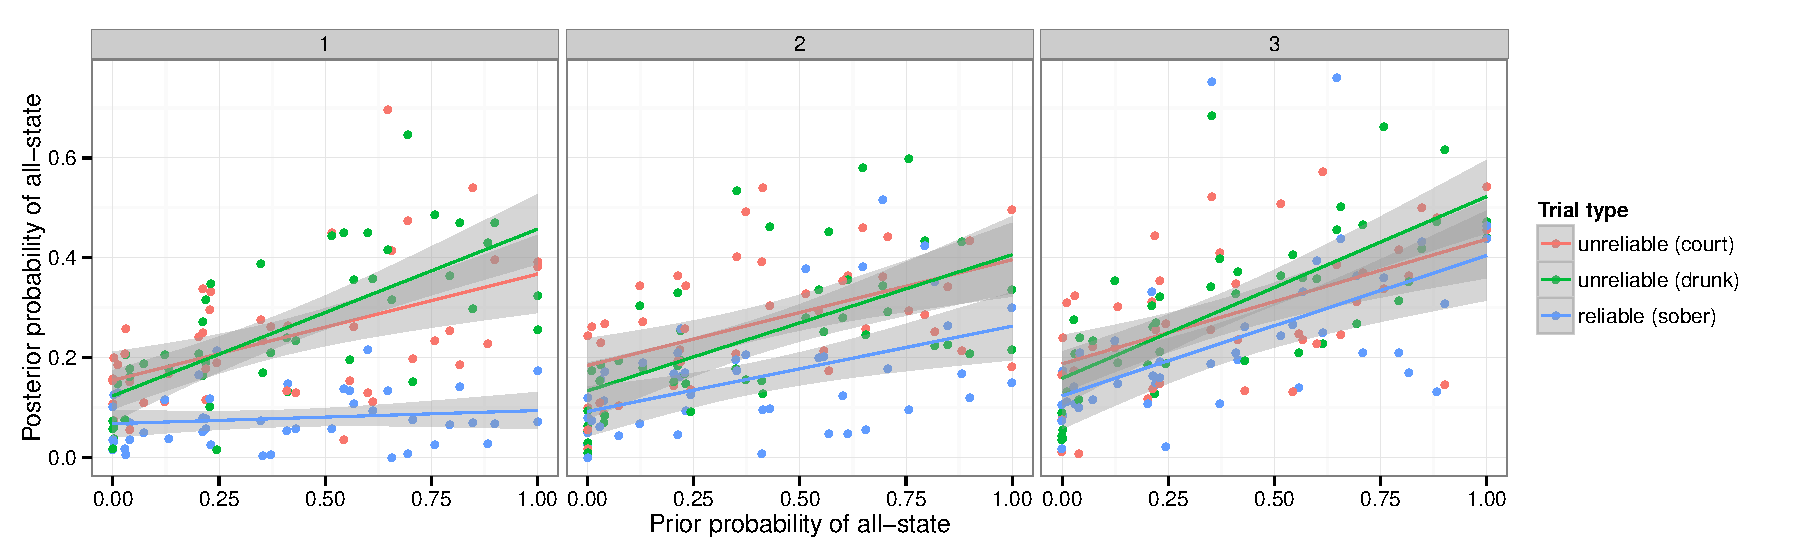
\includegraphics[width=\textwidth]{pics/speakerreliabilityresults-byblock}
	\caption{For each item, empirical mean posterior all-state probability against  prior all-state probability for reliable (\emph{sober}) and unreliable (\emph{drunk, court}) speakers, by experimental block. Reliable speakers are increasingly treated like unreliable speakers as the experiment progresses.}
	\label{fig:speakerreliability-byblock}	
\end{figure}

This is interesting because it suggests that listeners are drawing a higher-level inference about speakers being unreliable in this context (where the context may be this particular party, or  this particular experiment), such that participants who had evidence that there were unreliable speakers in this scenario also took the sober speaker less seriously.\footnote{Note that in principle the reverse could have happened, that is, evidence for the presence of reliable speakers could have resulted in treatment of the unreliable speakers as more reliable over time. We see no evidence for this.}  

Taken together, these results suggest that, as predicted, listeners more strongly take into account their prior beliefs when they interpret an utterance produced by an unreliable speaker than one produced by a reliable speaker. In addition, as evidence for unreliability of speakers accumulates, listeners generalize their expectation for unreliability even to a priori reliable speakers, resulting in a greater belief in listeners' priors.

% (Intercept)                               0.2351389  0.0129339  18.180
%cAllPriorProbability                      0.2618914  0.0310649   8.430
%cReliability                              0.1137068  0.0146606   7.756
%cTrial                                    0.0031160  0.0003527   8.834
%cAllPriorProbability:cReliability         0.1408706  0.0338892   4.157
%cAllPriorProbability:cTrial               0.0037873  0.0009860   3.841
%cReliability:cTrial                       0.0002214  0.0008919   0.248
%cAllPriorProbability:cReliability:cTrial -0.0009727  0.0022225  -0.438



\section{Discussion and conclusion}
\label{sec:gd}
% todo overhaul


%Interlocutors bring a wealth of world knowledge to bear on any language interpretation task. While effects of world knowledge in different areas of language processing are well-established (\red{psycholinguistics refs}), there has to date been a surprising lack of quantitative investigation into the role of world knowledge--and its defeasibility--in pragmatic inference. 
We have shown that listeners' world knowledge, in the form of prior beliefs, enters into the computation of speaker meaning in a systematic but subtle way. The effect of the prior on interpretation was much smaller, and qualitatively different, than predicted by a standard Bayesian model of quantifier interpretation (RSA). 
This suggests that in certain situations, listeners revise their assumptions about relevant priors as part of the computation of speaker meaning. 
Indeed, in the cases where the largest deviations from RSA obtained, participants also judged the world to be unusual.
%We have provided empirical evidence that the types of situations that lead to such revision , that is, situations in which the speaker's utterance is too unlikely given the listener's default prior beliefs and the available utterance alternatives. are cases of `wonky' worlds
Extending RSA with a lifted wonkiness variable that captures precisely whether listeners think the world is unusual, and allows them to back off to a uniform prior (i.e., ignore entirely their previously held beliefs about the world), provided a good fit to the empirical wonkiness judgments and dramatically improved the fit to participants' comprehension data. This model constitutes the first attempt to explicitly model the quantitative effect of world knowledge and its defeasibility on pragmatic utterance interpretation and raises many interesting questions.

In one sense the revision of beliefs in the wRSA listener is standard Bayesian belief updating with respect to a complex prior; however it is not the simple belief update of a flat or hierarchical prior, because the different aspects of prior belief (i.e.~$P(w)$ and $P(s|w)$) interact in complex ways with the listener's assumptions about the speaker.
As a result, an odd utterance can lead the listener to update their own view of $w$; this in turn impacts both their own prior over states and what prior they believe the speaker believes they are using---an odd utterance leads the listener to re-evaluate common ground. 
This is reminiscent of linguistic theories of presupposition accommodation \cite{lewis1979,stalnaker1973,stalnaker1998}.
It will be interesting to further explore the relation of the wRSA approach to presupposition.

Throughout this paper we discussed wonkiness as an attribute of the \emph{world}, yet empirically we elicited wonkiness judgments about the \emph{objects} involved in the events. 
This raises the question of what exactly listeners are revising their prior beliefs about: objects, events, the speaker's beliefs, or the way the speaker uses language?  For example % CONTINUE HERE
%Relatedly, in the current implementation of wRSA, prior belief revision has a global effect: that is, the prior that the listener infers is simultaneously the prior the listener attributes to the speaker; that is, the prior is treated as being in common ground, and the revision of the prior thus leads to a revision of common ground. But it is in fact an empirical question whether listeners revise their own privileged beliefs about the world, their beliefs about the common ground, or their beliefs about the speaker's beliefs. \red{WONKY SENTENCE: Addressing this question in future research will reveal whether a more complex mechanism for prior belief revision needs to incorporated that explicitly models prior vs.~privileged ground.}
Relatedly, we have used a uniform prior distribution as the alternative to consider when the listener believes the world is wonky.  One could imagine various more flexible alternatives. For instance, listeners may make minimal adjustments to their prior knowledge, or alternatively, may prefer extreme priors that rationalize the utterance once they have discounted the usual priors.
%Do metaphorical interpretations draw listeners out of the wonky world? 
Future research should investigate the options listeners have available when their world knowledge must be revised to accommodate an utterance.

This work also has methodological implications: researchers working in the field of experimental semantics and pragmatics would be well served to take into account the effect of `odd' items, prior beliefs, and interactions between the two.\footnote{For an in depth discussion of this issue in syntactic processing, see, e.g., \citeA{jaeger2010, fine2013a}.} In particular, if the attempt to design uniform stimuli across conditions yields odd utterances in some conditions, we predict that participants will respond by revising their prior beliefs in ways that can be unpredictable. That is, we expect unpredictable interaction effects between stimuli and conditions. This is likely to inflate or compress potential effects of an experimental manipulation. 

Concluding, this work exemplifies the importance and utility of exploring the detailed quantitative predictions of formal models of language understanding.
Exploring the prior knowledge effects predicted by RSA led us to understand better the influence of world knowledge and its defeasibility on pragmatic interpretation.
Listeners have many resources open to them when confronted with an odd utterance, and re-construing the situation %, rather than giving up the assumption of speaker cooperativity, 
appears to be a favorite.


%\begin{itemize}
%
%%	\item what is wonky? -- objects, event, speaker? -- connection to adaptation?
%%	\item other ways of asking about wonkiness
%%	\item \red{what's the right prior to back off to?}
%%	\item revising private beliefs vs revising common ground.
%%	\item \red{connection to presupposition (cf stalnaker), and other phenomena}
%%	\item implication for experiments on language understanding
%
%\end{itemize}

\appendix

\section{Items}
\label{sec:items}

\red{XXX}

\bibliographystyle{apacite}

\setlength{\bibleftmargin}{.125in}
\setlength{\bibindent}{-\bibleftmargin}

\bibliography{bibs}


\end{document}
